\documentclass[10pt, aspectratio=169]{beamer}
\usepackage{amsmath, amssymb, bm}
\usepackage{graphicx}
\usepackage{booktabs}
\usepackage{xcolor}

\graphicspath{{figures/}}

\usetheme{metropolis}
\setbeamertemplate{frame numbering}[fraction]

\newcommand{\xib}{\xi_b}
\newcommand{\ub}{u_b}
\newcommand{\vb}{v_b}

\title{Frequency-domain training data for a learned plasma fluid closure}
\subtitle{Tighter errors, $100\times$ cheaper data, same NN}
\author{Archis Joglekar}
\date{\today}

\begin{document}

\maketitle

% =================================================================
\begin{frame}{Setup: cold-bulk + warm-beam two-fluid}
  3-moment beam fluid coupled to cold bulk via Poisson:
  \begin{align*}
    \partial_t u   &= -E,\\
    \partial_t E   &= u - \varepsilon(\ub U_0 + U_1),\\
    \partial_t U_n &= -ik\ub U_n - ik U_{n+1} + n M_{n-1} E.
  \end{align*}

  \textbf{Closure problem:} need $U_3$ from $(U_0, U_1, U_2)$.

  \vspace{0.4em}
  \textbf{Kinetic linear response} (Maxwellian beam):
  \[
    U_0/\hat\Phi = Z'(\xib),
    \qquad \xib = \frac{\omega - k\ub}{k\vb}
  \]

  \textbf{Exact closure ratio:}
  \[
    \boxed{\;\alpha(\xib) \equiv U_3/U_0 = \xib^3 - \xib/Z'(\xib)\;}
  \]
\end{frame}

% =================================================================
\begin{frame}{Pad\'e baseline (HP / Hunana hierarchy)}
  \scriptsize
  Linear-in-moments closure $U_3 = \sum_i a_i U_i$ produces a degree-$(1,3)$
  rational of $Z'(\xib)$. Hunana et al.\ 2019: extended hierarchy up to 8 poles.
  \vspace{-0.4em}
  \begin{center}
    
\includegraphics[width=0.85\linewidth]{fig_response_function}
  \end{center}
  Residual $\sim\!10^{-2N+3}$ near origin, plateau at $\sim\!10^0$ for
  $|\xib|>1$: a fixed-order rational cannot match an entire function
  everywhere.
\end{frame}

% =================================================================
\begin{frame}{Pad\'e overshoot vs hierarchy order}
  \begin{columns}[T]
    \begin{column}{0.55\textwidth}
      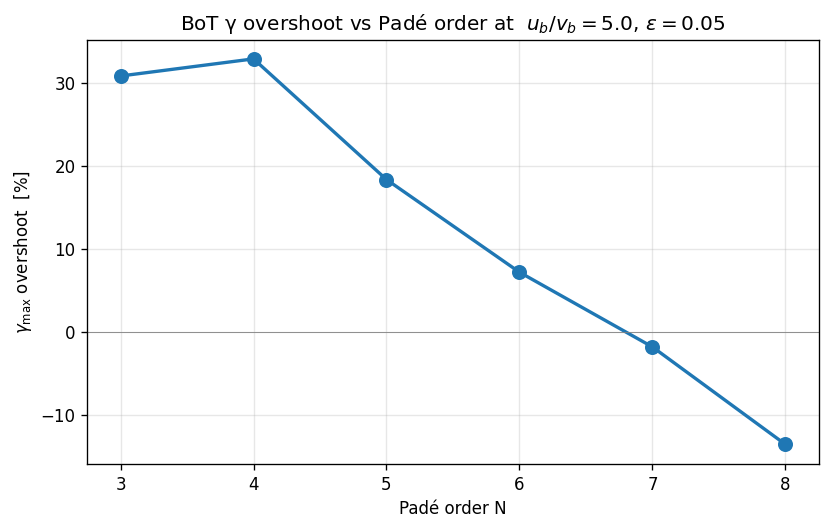
\includegraphics[width=\linewidth]{fig_overshoot_vs_N}
    \end{column}
    \begin{column}{0.45\textwidth}
      \footnotesize
      Canonical $(\ub/\vb, \varepsilon) = (5, 0.05)$:

      \vspace{0.5em}
      \begin{tabular}{lr}
        \toprule
        $N$ & overshoot \\
        \midrule
        3 & $+30.8\%$ \\
        4 & $+32.9\%$ \\
        5 & $+18.4\%$ \\
        6 & $+7.2\%$ \\
        7 & $-1.8\%$ \\
        8 & $-13.6\%$ \\
        \bottomrule
      \end{tabular}

      \vspace{0.6em}
      Crosses zero near $N\!=\!7$: classic non-monotone behaviour of
      rational approximation to a non-rational target.
    \end{column}
  \end{columns}
\end{frame}

% =================================================================
\begin{frame}{A structural identity: the per-mode closure in closed form}
  \footnotesize
  Before introducing the NN, one closed-form identity worth recording ---
  it determines what any closure must reduce to on a single eigenmode.
  The recurrence on a Maxwellian beam:
  \[
    U_{n+1} = \xib\, U_n - n M_{n-1}\Phih,
    \qquad M_0 = 1,\; \boxed{M_1 = 0}.
  \]
  Apply it three times:
  \begin{align*}
    U_1 &= \xib\, U_0\\
    U_2 &= \xib\, U_1 - M_0\,\Phih \;=\; \xib^2 U_0 - \Phih \quad\text{(since } M_0\!=\!1\text{)}\\
    U_3 &= \xib\, U_2 - 2 M_1 \Phih \;=\; \xib\, U_2 \quad \text{(since } M_1\!=\!0\text{)}
  \end{align*}
  Divide $U_3 = \xib U_2$ by $U_0$ and use $\xib = U_1/U_0$:
  \[
    \boxed{\;\alpha \;=\; \frac{U_3}{U_0} \;=\; \frac{U_1}{U_0}\cdot\frac{U_2}{U_0}\;}
  \]
  \emph{Exact per-eigenmode}, zero parameters. Verify directly:
  $r_1 r_2 = \xib(\xib^2 - 1/Z'(\xib)) = \xib^3 - \xib/Z'(\xib) = \alpha(\xib)$.
  All the $Z'$ machinery is absorbed into $U_2$; the closure step itself is
  complex multiplication.

  \vspace{0.4em}
  Used directly in time-domain it fails: a superposition of $N$
  eigenmodes gives $(\sum_i A_i U_1^{(i)})(\sum_j A_j U_2^{(j)}) \neq
  (\sum_k A_k U_0^{(k)})(\sum_\ell A_\ell U_3^{(\ell)})$ --- cross-terms
  break it. So this identity is not a usable time-domain closure.
  \emph{It's a constraint on what any per-mode closure must equal.}
  We will use it in two slides to ask: \emph{is this what the NN learned?}
\end{frame}

% =================================================================
\begin{frame}{NN closure: replace the linear closure}
  Replace $U_3 = \sum_i a_i U_i$ (constants) by
  \[
    \boxed{\;U_3 = f_\theta(U_1/U_0,\, U_2/U_0) \cdot U_0\;}
  \]
  with $f_\theta$ a small MLP. Nonlinear-in-moments, no rational-order
  ceiling.

  \vspace{1em}
  \textbf{Architecture (fixed throughout).}
  4-layer MLP, $(64,64,64,64)$ hidden, $\tanh$, $\sim\!8.7$k params.\;
  4 reals in (re/im of two complex moment ratios), 2 reals out (re/im of
  $\alpha$).

  \vspace{0.8em}
  \textbf{Question:} where does the training data come from?
\end{frame}

% =================================================================
\begin{frame}{Default: train on simulation trajectories}
  \footnotesize
  Standard recipe in data-driven closures:
  \begin{itemize}\itemsep0.15em
    \item Sweep $(\ub/\vb, \varepsilon, k, \mathrm{IC})$, integrate kinetic
          linear system in time.
    \item At each time step record $(U_0, U_1, U_2, U_3)$ along trajectory.
    \item Regress $U_3/U_0$ on $(U_1/U_0,\, U_2/U_0)$.
  \end{itemize}

  \vspace{0.3em}
  \textbf{Broad training sweep.}
  \begin{itemize}\itemsep0.1em
    \item $\ub/\vb \in \{3, 4, 5, 6, 8, 10\}$
    \item $\varepsilon \in \{0.02, 0.05, 0.10, 0.20\}$
    \item $5$ values of $k$ per op pt, $12$ random ICs each
    \item $\sim 10^5$ training samples after transient filtering
  \end{itemize}

  \vspace{0.4em}
  Designed to be \emph{broad} for maximum coverage.
\end{frame}

% =================================================================
\begin{frame}{Sim-trained NN: dispersion looks fine}
  \vspace{-0.5em}
  \begin{center}
    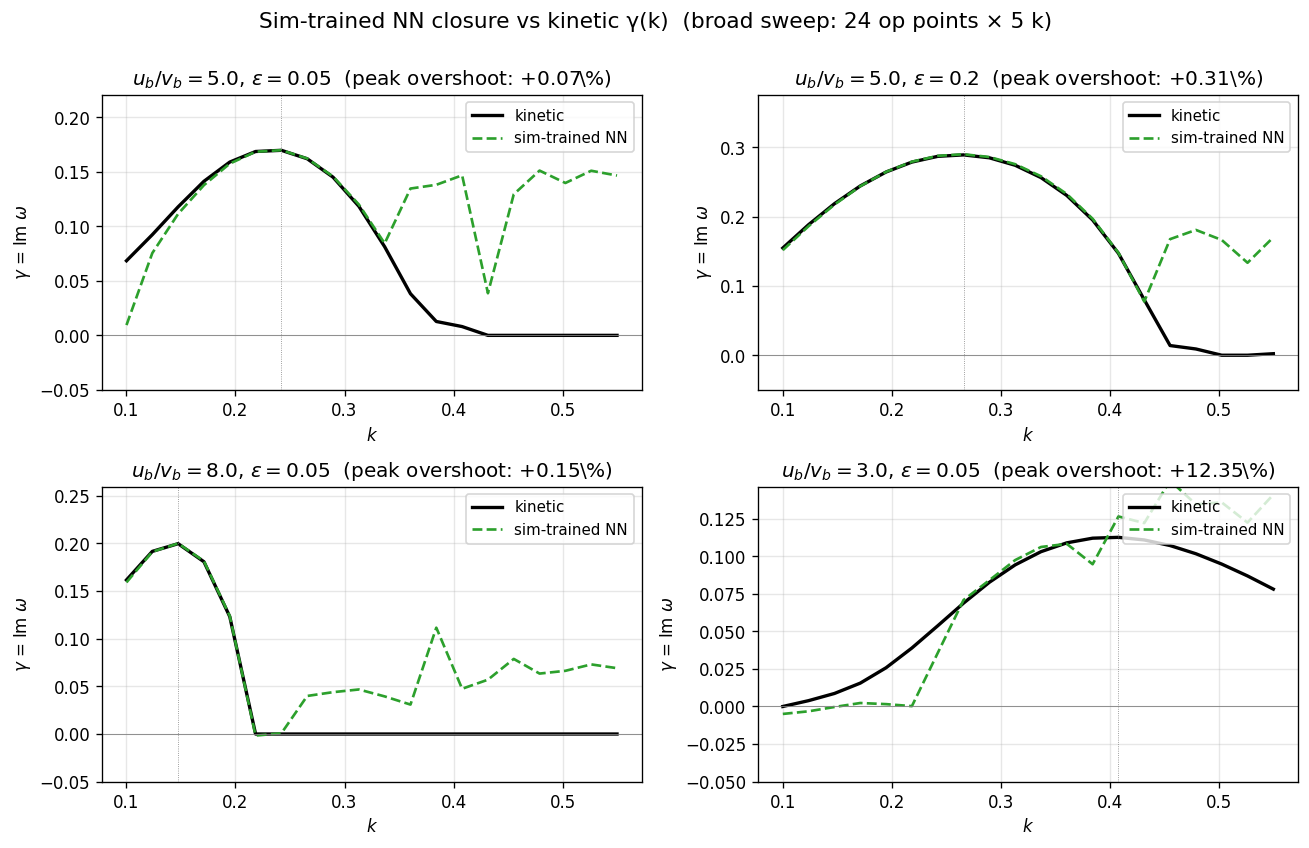
\includegraphics[width=0.62\linewidth]{fig_sim_dispersion}
  \end{center}
  \vspace{-0.4em}
  \scriptsize
  $\gamma(k)$ tracks kinetic through the unstable branch at $3/4$
  representative points; $\lesssim 1\%$ peak overshoot. Marginal corner
  $(3, 0.05)$ shows the first crack: $+12\%$.
\end{frame}

% =================================================================
\begin{frame}{Sim-trained NN: canonical time-domain looks fine}
  \vspace{-0.5em}
  \begin{center}
    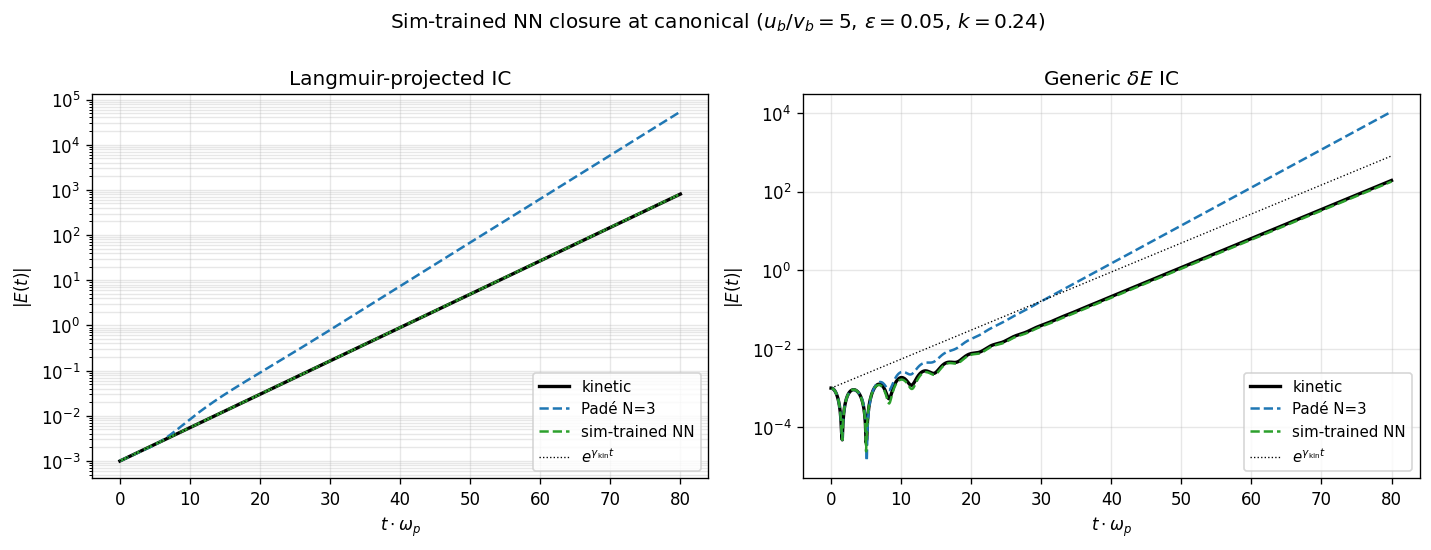
\includegraphics[width=0.85\linewidth]{fig_time_domain_sim}
  \end{center}
  \vspace{-0.4em}
  \scriptsize
  At $(5, 0.05, k\!=\!0.24)$: tracks kinetic under both Langmuir-projected
  and generic-$\delta E$ ICs. Fitted $\gamma_{\rm eff}\!=\!+0.1701$ vs
  $\gamma_{\rm kin}\!=\!+0.1700$. Canonical point is well inside training
  distribution.
\end{frame}

% =================================================================
\begin{frame}{Sim-trained NN: 2D scan}
  \vspace{-0.4em}
  \begin{center}
    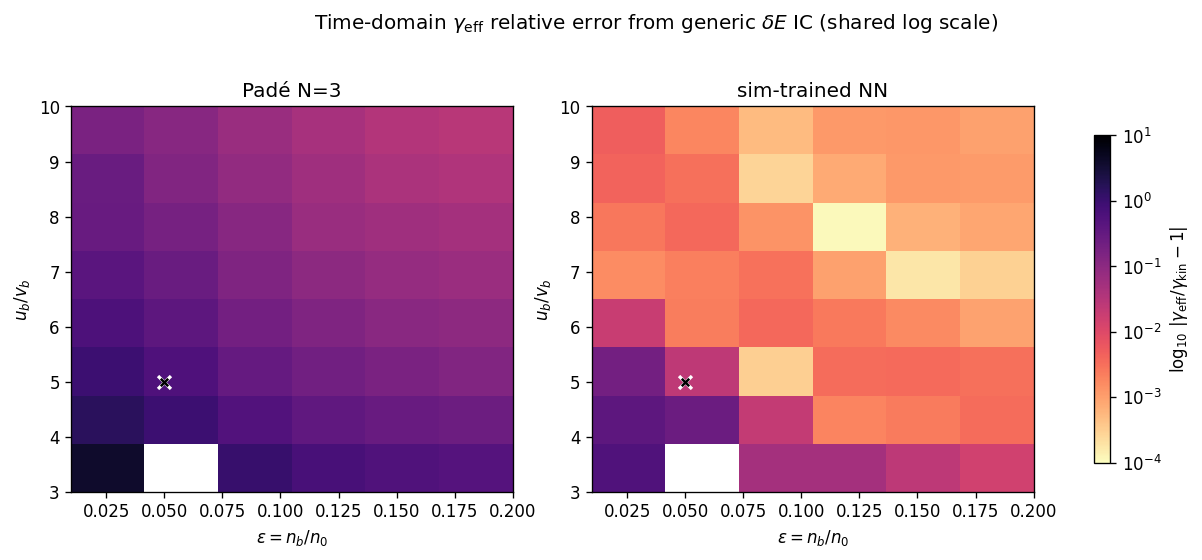
\includegraphics[width=0.78\linewidth]{fig_sweep_timedomain_sim}
  \end{center}
  \vspace{-0.5em}
  \scriptsize
  $\log_{10}|\gamma_{\rm eff}/\gamma_{\rm kin}-1|$, shared across all 2D
  sweeps. Sim-trained NN: one decade better than Pad\'e in the
  well-trained interior, $10^{-2}$--$10^{-1}$ most cells,
  $\sim\!10^{-0.3}$ at the marginal corner.

  \vspace{0.2em}
  Within $\sim\!10\%$ on $\gamma_{\rm eff}$ over most of the grid ---
  genuinely solid for $10^5$ sim samples. Can we do better, cheaper?
\end{frame}

% =================================================================
\begin{frame}{Diagnosis: where is the data in $\xib$?}
  \vspace{-0.4em}
  \begin{center}
    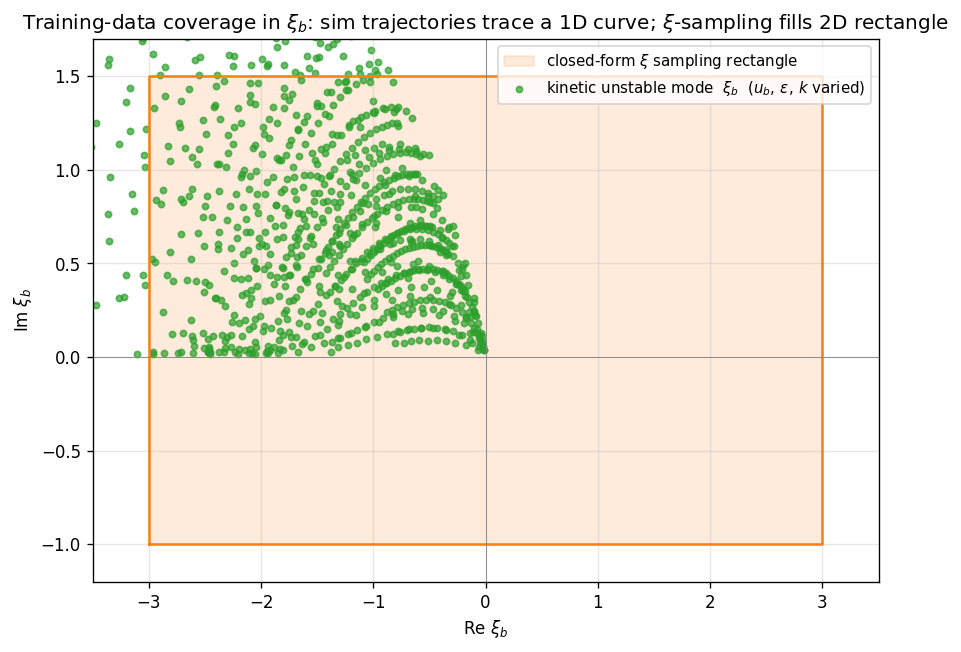
\includegraphics[width=0.62\linewidth]{fig_xi_coverage}
  \end{center}
  \vspace{-0.4em}
  \scriptsize
  $\xib$ on the unstable kinetic mode as $(\ub/\vb, \varepsilon, k)$ vary
  --- a narrow 1D-ish curve in the upper-left quadrant. The closed-form
  $\xib$ rectangle (orange) covers \emph{all} $\xib$ relevant for any
  fluid eigenmode (unstable + damped). Sim training never reaches the
  rest.
\end{frame}

% =================================================================
\begin{frame}{What the gradient is telling us}
  \footnotesize
  Generic $\delta E$ IC excites \emph{all five} fluid eigenmodes ---
  Langmuir-like plus four others. Their $\xib$ projections land all over
  the rectangle.

  \vspace{0.4em}
  \begin{itemize}\itemsep0.15em
    \item Sim training sees only the unstable Langmuir mode's $\xib$.
    \item Other modes evaluated at moment ratios off the green curve
          $\Rightarrow$ NN extrapolates $\alpha$.
    \item When extrapolation is benign (canonical, hot beam) the trajectory
          still settles to $\gamma_{\rm kin}$; when it isn't (marginal
          corner) the error grows.
  \end{itemize}

  \vspace{0.4em}
  \textbf{The error gradient in the heatmap is the gradient of NN
  extrapolation quality.} More simulations don't change it: trajectories
  live on the eigenmode manifold; their $\xib$-projection \emph{is} the
  green region.
\end{frame}

% =================================================================
\begin{frame}{Fix: sample $\xib$ directly}
  \footnotesize
  Moment ratios on a linear eigenmode are closed-form in $\xib$ via the
  recurrence $U_{n+1} = \xib U_n - n M_{n-1}\hat\Phi$:
  \[
    U_1/U_0 = \xib, \qquad U_2/U_0 = \xib^2 - 1/Z'(\xib),
    \qquad \alpha = \xib^3 - \xib/Z'(\xib)
  \]
  One Faddeeva evaluation per training pair. No simulation required.

  \vspace{0.5em}
  \textbf{Sample uniformly:} $\xib$ in
  $\mathrm{Re}\,\xib\in[-3,3]$, $\mathrm{Im}\,\xib\in[-1,1.5]$. $16{,}384$
  samples.

  \vspace{0.5em}
  \textbf{Cost.} $\sim$\,0.1\,s of \texttt{scipy.special.wofz} vs minutes
  of kinetic integration for $\sim 10^5$ sim samples --- $\sim\!100\times$
  cheaper, no op-pt sweep, no ICs, no outlier filtering, no operating
  regime to choose.

  \vspace{0.3em}
  \textbf{Same physics, same NN, same training schedule.} Only the data
  changes.
\end{frame}

% =================================================================
\begin{frame}{Off-mode $\alpha$ accuracy: sim vs $\xib$-sampling}
  \begin{center}\small
  \begin{tabular}{lccc}
    \toprule
    $\xib$ & sim (1 op pt) & sim (broad, 24) & closed-form \\
    \midrule
    $-1.17 + 0.71i$ (eigenmode) & $+2.3\%$  & $+0.8\%$  & $+0.05\%$ \\
    $-0.83 + 0.05i$ & $+148\%$  & $+62\%$   & $+0.5\%$ \\
    $0.50 + 0.00i$  & $+843\%$  & $+247\%$  & $+0.6\%$ \\
    $-1.50 - 0.20i$ & $+50\%$   & $+27\%$   & $+0.2\%$ \\
    $1.20 + 0.10i$  & $+209\%$  & $+118\%$  & $+0.6\%$ \\
    $-2.00 + 0.00i$ & $+13\%$   & $+7\%$    & $+0.5\%$ \\
    \bottomrule
  \end{tabular}
  \end{center}
  \vspace{0.4em}\footnotesize
  $|\alpha_{\rm NN} - \alpha_{\rm exact}|/|\alpha_{\rm exact}|$ at test
  $\xib$. Sim training fits only the unstable curve; $\xib$-sampling is
  uniformly accurate.
\end{frame}

% =================================================================
\begin{frame}{$\gamma_{\max}$ sweep: $\xib$-sampled NN vs Pad\'e}
  \vspace{-0.4em}
  \begin{center}
    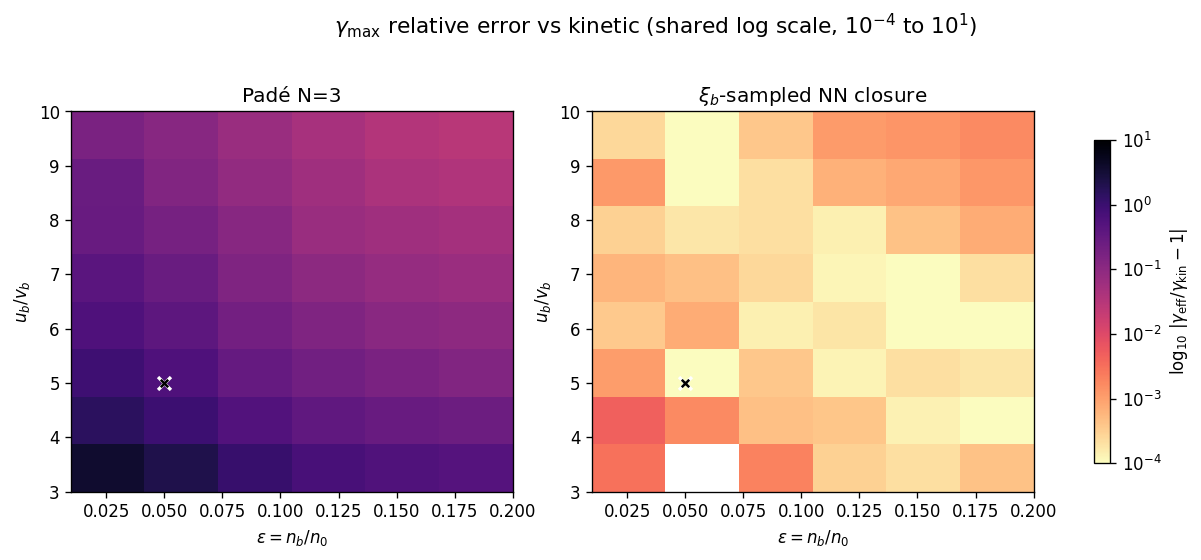
\includegraphics[width=0.82\linewidth]{fig_sweep_comparison}
  \end{center}
  \scriptsize
  Same log scale. Pad\'e $N\!=\!3$ sits at $10^{-1}$--$10^{0}$;
  $\xib$-sampled NN is $\le\!10^{-3}$ nearly everywhere. Two decades
  better than sim-trained, three to four decades better than Pad\'e.
\end{frame}

% =================================================================
\begin{frame}{Time-domain stress test ($\xib$-sampled NN)}
  \vspace{-0.4em}
  \begin{center}
    
\includegraphics[width=0.78\linewidth]{fig_time_domain}
  \end{center}
  \vspace{-0.4em}
  \scriptsize
  Generic $\delta E$ IC, $(5, 0.05, k\!=\!0.24)$. Fitted $\gamma_{\rm eff}$
  (Langmuir / generic): kinetic $+0.1700/+0.1700$, Pad\'e $+0.2223/+0.2223$,
  \textbf{$\xib$-sampled NN $+0.1700/+0.1700$}.
\end{frame}

% =================================================================
\begin{frame}{Time-domain 2D sweep: Pad\'e, bilinear identity, NN}
  \vspace{-0.4em}
  \begin{center}
    
\includegraphics[width=0.99\linewidth]{fig_sweep_timedomain_three}
  \end{center}
  \vspace{-0.4em}
  \scriptsize
  Pad\'e and the bare bilinear identity are visually indistinguishable
  on the shared log scale --- bilinear is a strict but small
  improvement ($\sim\!10\%$ relative reduction at canonical, larger only
  at the marginal corner where both are already deep into failure).
  The $\xib$-sampled NN is two to three decades tighter across the
  entire grid. \emph{Being structurally correct per-mode is not enough;
  the off-manifold behaviour is what makes the NN work.}
\end{frame}

% =================================================================
\begin{frame}{What is the NN doing? Off-manifold diagnostic}
  \vspace{-0.5em}
  \begin{center}
    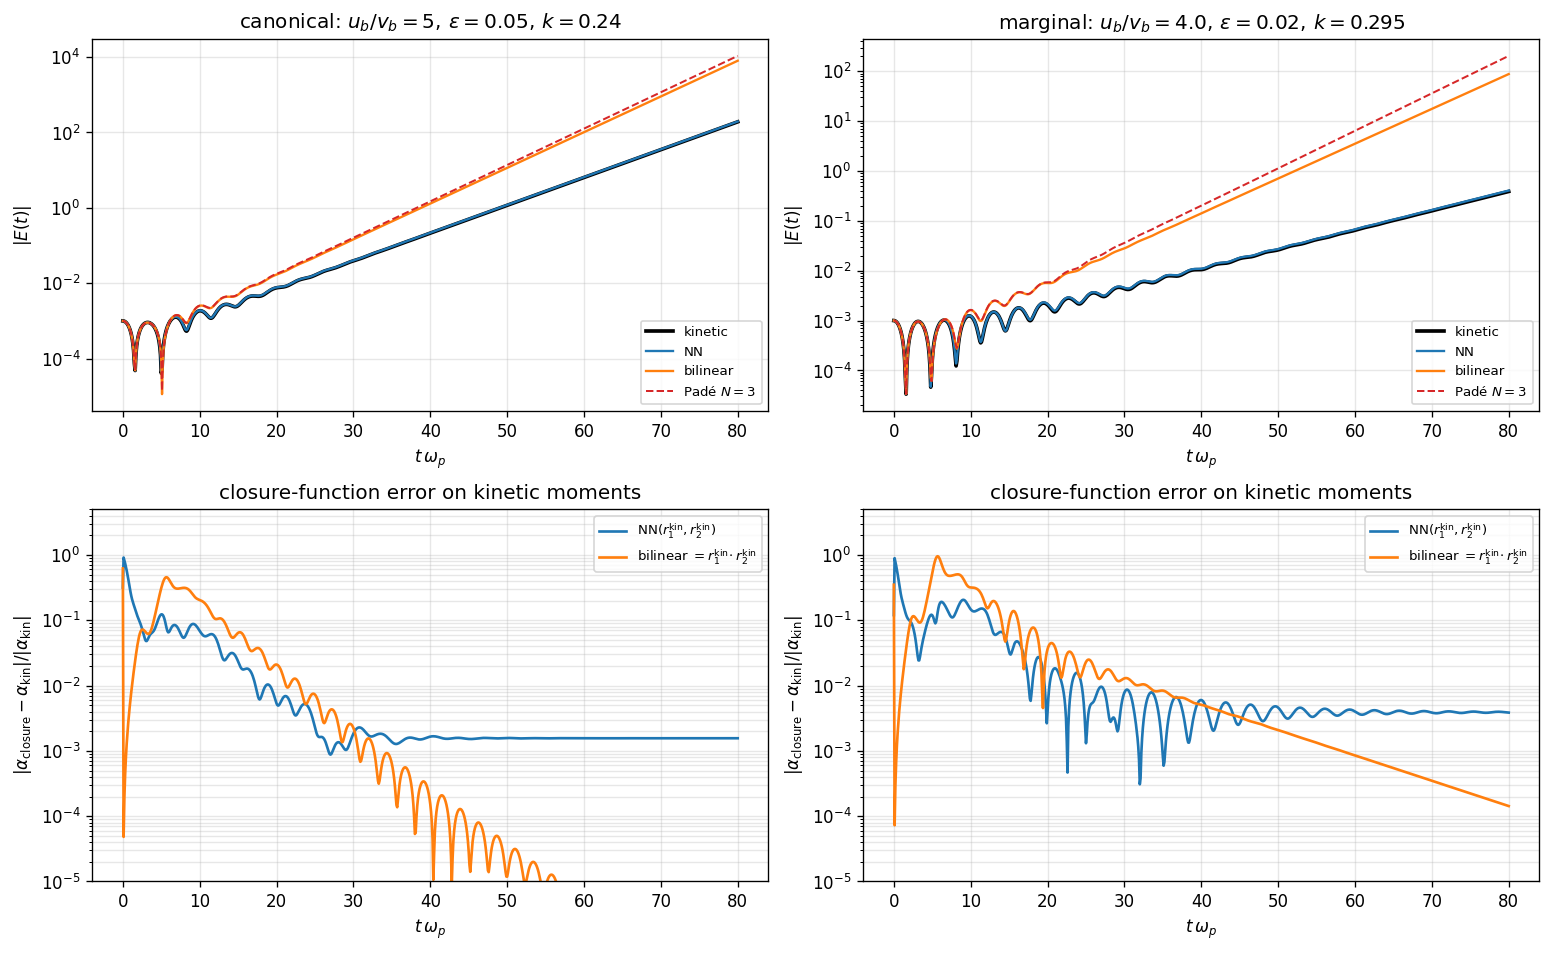
\includegraphics[width=0.85\linewidth]{fig_offmanifold_diagnostic}
  \end{center}
  \vspace{-0.4em}
  \scriptsize
  \textbf{Top}: $|E(t)|$. Bilinear (orange) tracks Pad\'e, not kinetic.
  \textbf{Bottom}: closure-function error $|\alpha_{\rm closure} - \alpha_{\rm kin}|/|\alpha_{\rm kin}|$
  evaluated on the \emph{kinetic} moments (isolates the closure function
  from trajectory feedback).

  \vspace{0.3em}
  \emph{Early time} (multimode): NN at $\sim\!10^{-2}$; bilinear at
  $10^{-1}$--$10^{0}$. NN is the better off-manifold closure.\\
  \emph{Late time} (mode-dominated): bilinear falls to $10^{-5}$ ---
  per-mode identity is exact; NN plateaus at $10^{-2}$ residual training
  error. Bilinear actually beats NN here.

  \vspace{0.3em}
  Mechanism: a single early-time mis-fire seeds spurious closure modes
  that grow exponentially. The NN's off-manifold accuracy in the
  multimode phase \emph{locks the trajectory onto the kinetic eigenmode}
  before that happens; bilinear can't.
\end{frame}

% =================================================================
\begin{frame}{What did the NN learn?}
  \footnotesize
  Off-manifold check: evaluate $f_\theta(r_1, r_2)$ at $(r_1, r_2)$ drawn
  \emph{independently} from the on-manifold bounding box (not consistent
  with any single $\xib$).
  \begin{center}
  \begin{tabular}{lcc}
    \toprule
    sample location & $|f_\theta - r_1 r_2|/|r_1 r_2|$ (mean) \\
    \midrule
    on eigenmode manifold (training) & $3 \times 10^{-3}$ \\
    off manifold (independent $r_1, r_2$) & $\sim\!1$ \\
    \bottomrule
  \end{tabular}
  \end{center}

  \vspace{0.4em}
  The NN did \emph{not} learn complex multiplication globally. It learned a
  particular smooth interpolation in $(r_1, r_2)$-space that
  \begin{itemize}\itemsep0.1em
    \item matches the bilinear product on the 2-real-d eigenmode submanifold
          (where it was trained), and
    \item happens, off-manifold, to suppress superposition cross-term error.
  \end{itemize}

  \vspace{0.4em}
  \emph{Per-mode}, the structurally correct closure is bilinear (provable).
  \emph{On a real trajectory}, the NN's smooth off-manifold extension is
  what makes the closure stable. Hardcoded multiplication is the wrong
  extension; the NN found a useful one.
\end{frame}

% =================================================================
\begin{frame}{Generalization: same NN, Landau damping}
  \footnotesize
  The trained closure depends only on the Maxwellian linear response ---
  no $\ub$, $\varepsilon$, $k$ in the training data. Should work for any
  3-moment Maxwellian-fluid setup. Test: Langmuir wave on a single warm
  Maxwellian, no beam, no cold bulk. Strip BoT to:
  \[
    \partial_t E = -U_1, \quad
    \partial_t U_0 = -ik U_1, \quad
    \partial_t U_1 = -ik U_2 + E, \quad
    \partial_t U_2 = -ik U_3.
  \]
  Same checkpoint. No retraining.
  \vspace{-0.6em}
  \begin{center}
    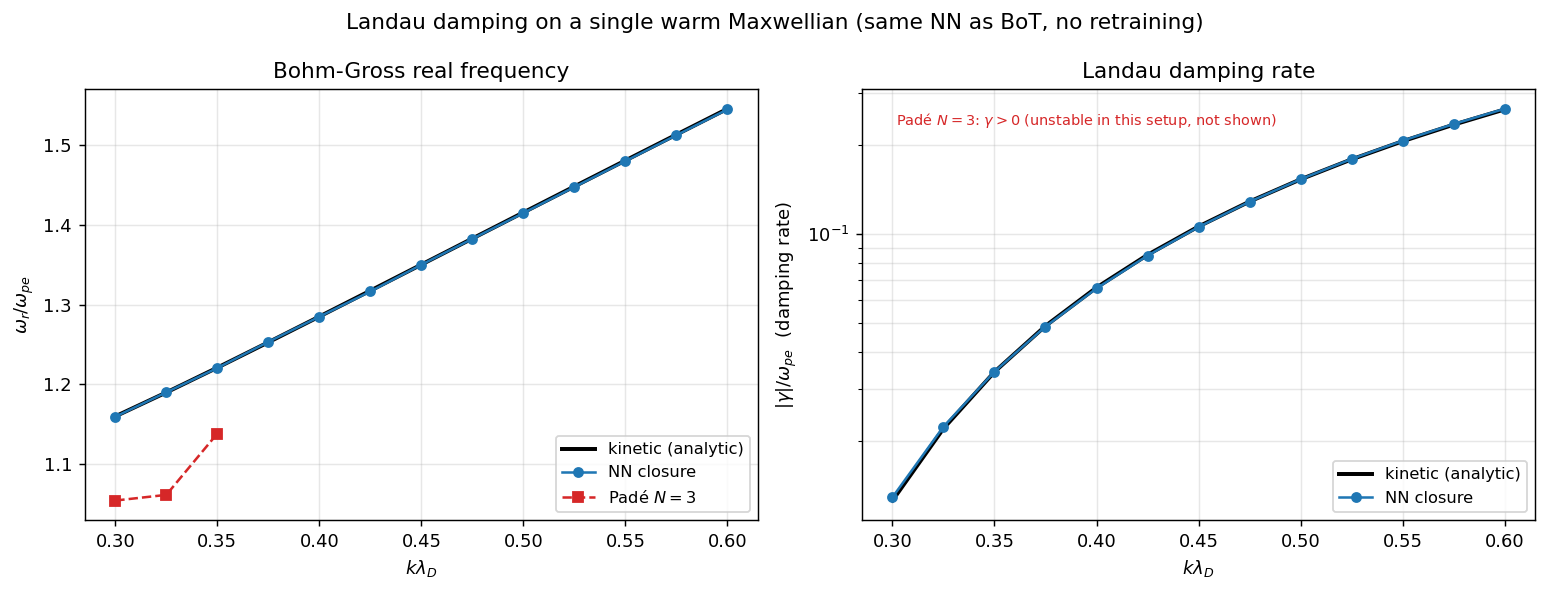
\includegraphics[width=0.98\linewidth]{fig_landau_damping}
  \end{center}
  \vspace{-0.6em}
  NN matches kinetic Landau rate to $\le\!1\%$ across $k\lambda_D \in
  [0.3, 0.6]$ ($\gamma/\omega_{pe} = -0.0126, -0.066, -0.153, -0.264$
  at $k\lambda_D = 0.3, 0.4, 0.5, 0.6$ --- textbook values). Pad\'e is
  \emph{unstable} on this setup ($\gamma > 0$) --- a known issue with
  Taylor-matching closures without cold-bulk grounding.
\end{frame}

% =================================================================
\begin{frame}{Headline}
  \footnotesize
  \textbf{Closure result.} $\xib$-sampled NN gives $10^{-4}$--$10^{-3}$
  relative error on $\gamma_{\rm eff}$ across the $(\ub/\vb, \varepsilon)$
  grid --- two decades tighter than sim-trained, three to four decades
  tighter than Pad\'e. Data is $16{,}384$ Faddeeva evaluations,
  $\sim\!100\times$ cheaper than sim sampling, problem-agnostic.

  \vspace{0.4em}
  \textbf{Generalization.} Same checkpoint, no retraining, reproduces
  Landau damping on a single warm Maxwellian to $<\!1\%$ across
  $k\lambda_D \in [0.3, 0.6]$. The closure object is a learned Maxwellian
  linear-response function, reusable for \emph{any} 3-moment fluid
  integrator on a Maxwellian equilibrium (BoT, Langmuir damping,
  ion-acoustic, drift waves).

  \vspace{0.5em}
  \textbf{Interpretability.} A one-line algebraic identity from the
  recurrence + $M_1\!=\!0$ pins the exact per-mode closure to a complex
  product, $\alpha = (U_1/U_0)(U_2/U_0)$. The NN reproduces this on the
  eigenmode manifold (where it was trained) but does \emph{not} learn
  multiplication globally --- off the manifold it produces a smooth
  interpolation that is distinctly non-multiplicative. Hardcoding
  multiplication directly produces a closure that fails almost as badly
  as Pad\'e on generic ICs (cross-terms break the identity). The
  off-manifold smooth extension --- not the on-manifold identity --- is
  what makes the NN closure work.

  \vspace{0.3em}
  \begin{center}
    \emph{Same NN. Strictly better data.\\
    Mechanism: per-mode product on the manifold, useful smooth
    extension off it.}
  \end{center}
\end{frame}

\end{document}
